\chapter{Related Work}

This chapter gives a review of a few projects that are related to this work. The first section deals with projects that have as objective the securing of passwords using a hardware approach. The second section regards applications using the SEcube™ framework.

\section {Hardware Password Wallets}
Over the last decade, ... 

\subsection {Mooltipass: A Simple Offline Password Keeper} 

The Mooltipass is a hardware-based password keeper commercial product that allows users to safely carry their credentials with them all the time, and use them when needed by connecting a portable device to a computer and authenticating using a 4 characters pin. 
Figure \ref{fig:mool} depicts the mooltipass system.

\begin{figure}[htb]
  \centering
  \captionsetup{justification=centering}
  \centerline{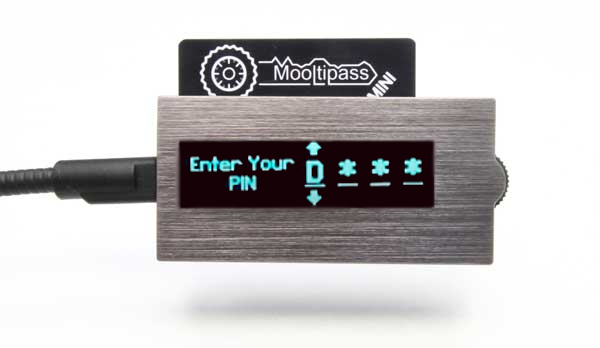
\includegraphics[width=0.6\columnwidth]{chapters/figures/related/mooltipass.jpg}}
  \caption{The mooltipass device and smartcard}
  \label{fig:mool}
\end{figure}

Its use is very, simple, as explained in their official website \cite{mooltipass}:

``The Mooltipass is designed to be as simple as possible to use for users of all backgrounds and ages:
\begin{enumerate}
\setlength\itemsep{0pt}
\item Plug the Mooltipass to your computer/tablet/phone. No driver is required
\item Insert your smartcard, unlock it with your PIN. Without the PIN, the card is useless.
\item Visit a website that needs a login. If using our browser plugin, the Mooltipass asks your permission to send the stored credentials, or asks you to save new ones if you are logging in for the first time.
\item If you are not using the browser plugin or are logging in on something other than a browser, you can tell the Mooltipass to type your logins and passwords for you, just like a keyboard.
\end{enumerate}

The Mooltipass emulates a standard USB keyboard, and can therefore type your passwords for you on Windows, Linux, Mac and even most Apple and Android devices (through the USB On-The-Go port). It doesn't need any special drivers to function. ''

The browser plugins offer a GUI where the user see and manage their passwords, as shown in Figure \ref{fig:mpapp}

\begin{figure}[htb]
  \centering
  \captionsetup{justification=centering}
  \centerline{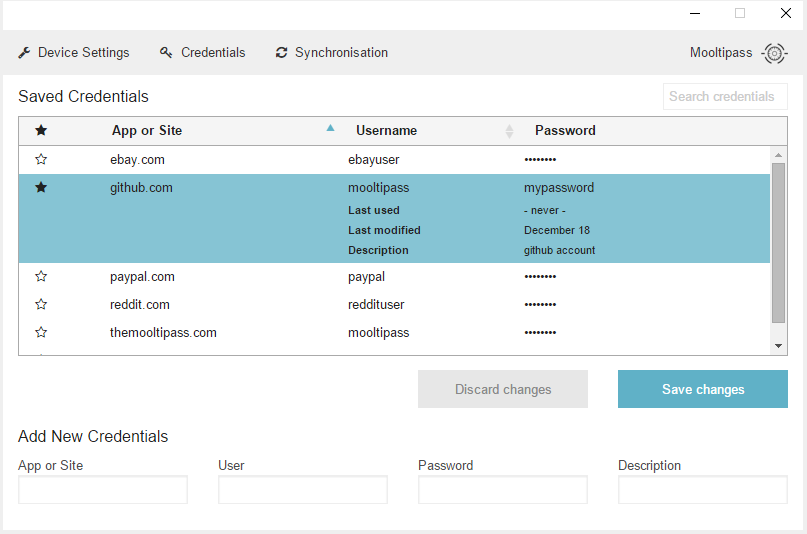
\includegraphics[width=0.9\columnwidth]{chapters/figures/related/mpapp.png}}
  \caption{The mooltipass application}
  \label{fig:mpapp}
\end{figure}

The Mooltipass works by storing an encrypted version of the passwords, and allowing their decryption only when the proper smartcard is connected and the correct pin introduced. From the website:

``The Mooltipass has an internal flash in which the user encrypted credentials are stored, while a PIN-locked smartcard contains the AES-256bits key required for their decryption. Like any chip and pin card, 3 false tries will permanently disable the Mooltipass card. Credentials are sent over HID, any password accessing operation needs to be physically approved by the user on the device.''

Mooltipass is open software and open hardware. In fact they encourage the community to develop and review code, so that the system's reliability is increased. Their GitHub repository host all the sources from the beginning of the project. \cite{mpgit}.

The Mooltipass project started off as a Hackday post from developer Mathieu Stephan, that gained enough recognition by the community to be founded by a kickstarter campaign. The Hackday project website \cite{mphack} contains more details regarding the hardware implementation:

\begin{itemize}
\setlength\itemsep{0pt}
\item \textbf{ST662ACD-TR:} Power Management
\item \textbf{ATMEGA32U4-MU:} Arduino compatible Microprocessor
\item \textbf{AT88SC102:} Secure Memory Smart Card
\item \textbf{AT45DB011D-SSH-T:} FLASH Memory
\end{itemize}

Figure \ref{fig:mparchi} shows the basic architecture.
\begin{figure}[htb]
  \centering
  \captionsetup{justification=centering}
  \centerline{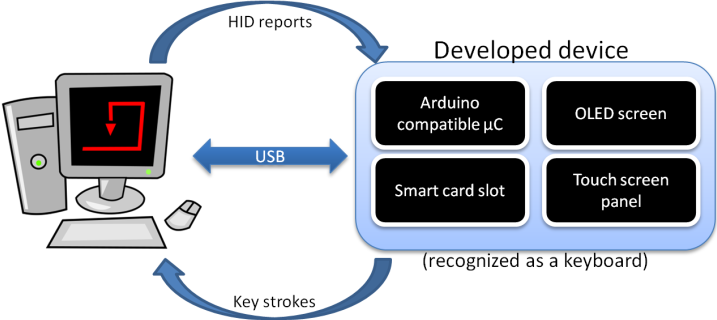
\includegraphics[width=0.9\columnwidth]{chapters/figures/related/mparchi.png}}
  \caption{The Mooltipass basic architecture}
  \label{fig:mparchi}
\end{figure}

In conclusion, mooltipass is a mature project that follows the same idea developed in this work: Guarantee the security of a set of passwords by allowing their decryption only through the use of a hardware device that the user will carry with them, hopefully, all the time. However there are some important difference between their system and SEcubeWallet:
\begin{enumerate}
\setlength\itemsep{0pt}
\item SEcubeWallet is based on the SEcube™ platform, making it much more trustworthy and robust, as this is a platform even used in military applications, and has been tested in the most demanding conditions.

\item Because SEcube™ integrates all the required security elements into one single chip, the final product is much more smaller (The size of a regular USB stick) than the mooltipass device.

\item Because the SEcube™ platform offers more possibilities for the development of applications, for example using the open source libraries, or the FPGA inside the chip, the SEcubeWallet can be extended or be integrated with other projects.

\item SEcubeWallet offers a couple of additional functionalities: Strong Password generation and entropy estimation, increasing the user experience.
\end{enumerate}

\section{SEcube™ based applications}

Before starting the application development, the following three projects were studied in order to familiarize with the SEcube™ framework and libraries usage. All of the projects make part of the SEfile SDK available at \cite{SEcubeRes} and are covered in details in the L2 user Manual \cite{L2UserMan}.

\subsection{Secure Text Editor and Secure Image Viewer}

This two projects are very similar, both use the SEcube™ framework, in particular the \texttt{SEfile} library, to encrypt/decrypt plain text files and images respectively. They are not intended to be final user applications, but demos that allow developers to learn how to use the SEcube™ libraries.

``Both these two projects have been developed in C++ with Qt libraries. They are based on 3
major security classes, in a one-to-one mapping with the 3 most important security opera-
tions: the first one manages the security platform to which the user wants to log in, the sec-
ond one allows the selection of the secure environment through the \texttt{secure\_update()} function, while the third one manages the opening and creation of files resorting on the \texttt{secure\_ls()}.''\citep{L2UserMan}.

The secure text editor, in short \texttt{SEfile\_TXT} offers the possibility to create/edit/open plain text documents, and generate an encrypted version of the file that will be stored in the same directory. ``It is possible to verify that encrypted files cannot be read properly from regular text editors; conversely, the Secure Text Editor can transparently read any encrypted file (decrypting also the file name) which content has not been altered and is, thus, trusted. Unauthenticated content (i.e., content not corresponding to the file signature) is, instead, discarded''.

The secure image viewer, in short \texttt{SEfile\_IMG} allows the user to open the most common image formats, PNG JPG/JPEG and BMP, and generates the encrypted version, which can only be opened using the same application.

Figure \ref{fig:sefiledem} depicts these two demo applications.

\begin{figure}[ht]
  \centering
  \subfloat[SEfile\_TXT demo application\label{}]{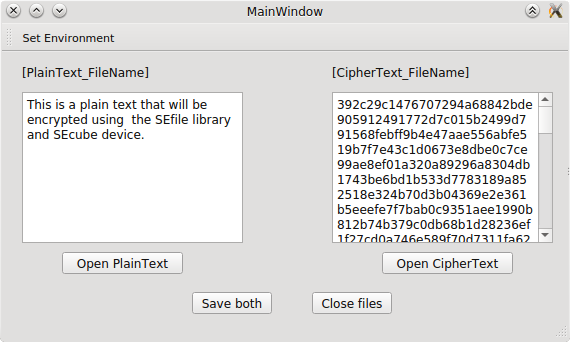
\includegraphics[width=0.48\textwidth]{chapters/figures/related/sefiletxt.png}}
  {}
  \subfloat[SEfile\_IMG\label{}]{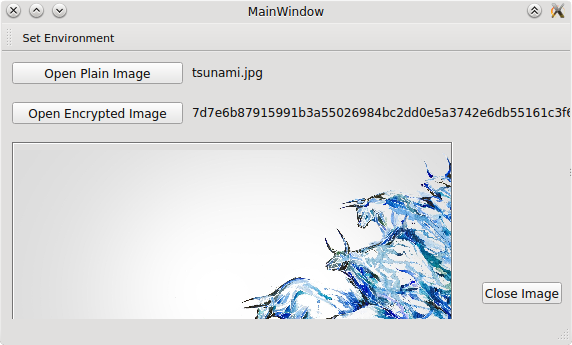
\includegraphics[width=0.48\textwidth]{chapters/figures/related/sefileimg.png}}
  \caption{SEfile demo applications}
 \label{fig:sefiledem}
\end{figure}

These two demo applications were used to learn the basis of the SEcube™ libraries, specially how to open the communication with the device, how to authenticate (login) and how to logout. The login dialogue used in the SEcubeWallet application is an improved version of these demos' login dialogue. The environmental dialogue was borrowed without any modification.

\subsection{secureSQLiteBrowser}

This application integrates the SEcube™ secureSQLite library with the DB Browser for SQLite\cite{SQLitebro} project, resulting in a powerful manager of encrypted SQLite databases.

The secureSQLite library, that makes part of the SEfile SDK, modifies the SQLite system to use the SEfile library in order to manage files, rather than using directly the OS calls. The result is a library that accepts all the standard SQLite commands, but stores the database as an encrypted file.

DB Browser for SQLite is an application developed in Qt that allows to manage SQLite DB from a powerful GUI. ``DB Browser for SQLite is a high quality, visual, open source tool to create, design, and edit database files compatible with SQLite. It is for users and developers wanting to create databases, search, and edit data. It uses a familiar spreadsheet-like interface, and you don't need to learn complicated SQL commands.'' \cite{SQLitebro}

By merging this two projects, the result is a wonderful application to create encrypted SQLite databases using an elegant and powerful GUI, depicted in figure \ref{fig:sqlitebro}, with tons of options, where the users can visually edit the DB tables, and store them as SEcube™ secured files. 

\begin{figure}[htb]
  \centering
  \captionsetup{justification=centering}
  \centerline{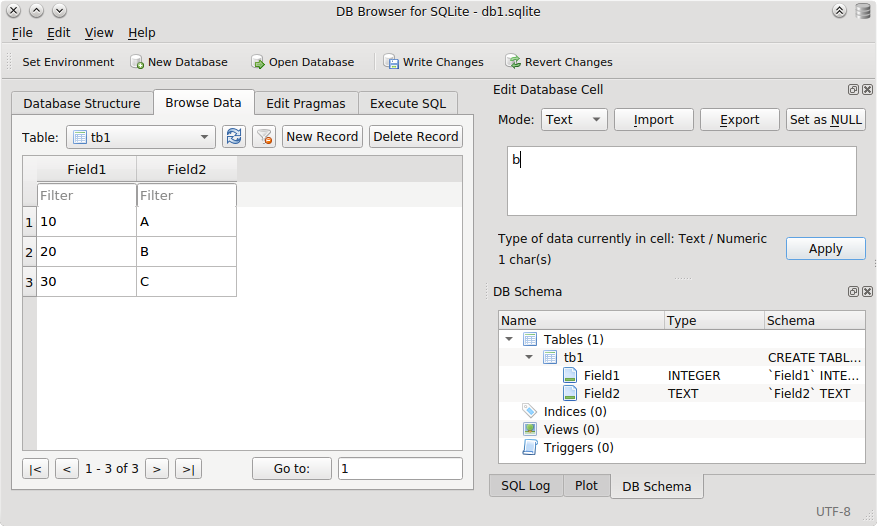
\includegraphics[width=1\columnwidth]{chapters/figures/related/sqlitebro.png}}
  \caption{secureSQLiteBrowser GUI}
  \label{fig:sqlitebro}
\end{figure}

Because SEcubeWallet is heavily based on the use of the secureSQLite library, this application was used to learn how to integrate the library into a Qt project. Additionally, it was used as inspiration for some of the GUI elements, like the filters above each column and the use of menus and toolbars. It was also use to diagnose the SEcubeWallet in the developing stage, by creating a DB with one application and opening it in the other. secureSQLiteBrowser could be use as a password manager in the sense that it can securely store and display wallets as tables, but it lacks the simplicity and additional functionalities that make SEcubeWallet attractive to users.



























